\input{./econtexRoot.texinput}
\documentclass[\econtexRoot/Chp1proposal]{subfiles}
\onlyinsubfile{\externaldocument{\econtexRoot/Chp1proposal}} % Get xrefs -- esp to apndx -- from main file; only works if main file has already been compiled

\begin{document}

\onlyinsubfile{\setcounter{section}{2}}
\section{Incorporating life cycle dynamics into the model}
\notinsubfile{\label{sec:Model}}

\par More realistic assumptions regarding the age and education level of households can have important implications for the income and mortality process of households. Here, I extend the model to incorporate these life cycle dynamics.

\par Households enter the economy at time $t$ aged 24 years old and are endowed with an education level $e \in \{D,HS,C\}$, and initial permanent income level $\textbf{p}_0$, and a capital stock $k_0$. The life cycle version of household income is given by:

$$ y_t = \xi_t \textbf{p}_t = (1 - \tau) \theta_t \textbf{p}_t, $$

where $\textbf{p}_t = \psi_t \bar{\psi}_{es} \textbf{p}_{t-1}$ and $\bar{\psi}_{es}$ captures the age-education-specific average growth factor. Households that have lived for $s$ periods have permanent shocks drawn from a lognormal distribution with mean $1$ and variance $\sigma^{2}_{\psi s}$ and transitory shocks drawn from a lognormal distribution with mean $\frac{1}{\cancel{\mho}}$ and variance $\sigma^{2}_{\theta s}$ with probability $\cancel{\mho} = (1-\mho)$ and $\mu$ with probability $\mho$.

\par The normalized version of the age-education-specific consumption-saving problem for households is given by

\begin{eqnarray*}
  v_{es}(m_t) &=& \max_{c_t} u(c_t(m_t)) + \beta \cancel{D}_{es} \mathbb{E}_{t}[\psi_{t+1}^{1-\rho}v_{es + 1}(m_{t+1})] \\
  &\text{s.t.}& \\
  a_t &=& m_t - c_t, \\
  k_{t+1} &=& \frac{a_t}{\psi_{t+1}}, \\
  m_{t+1} &=& (\daleth + r_t)k_{t+1} + \xi_{t+1}, \\
  a_t &\geq& 0.
\end{eqnarray*}

\subsection{Results}

\par The additional parameters necessary to calibrate the life cycle version of the model are given in table \ref{tab:calib2}.

\hypertarget{calibLC}{}
\begin{table}[ht]
  \centering
  \resizebox{0.6\textwidth}{!}{
    \begin{tabular}{ccc}
        \toprule
        Description & Parameter & Value  \\
        \midrule
        Population growth rate & $N$ & 0.0025  \\
        Technological growth rate & $\Gamma$ & 0.0037  \\
        Rate of high school dropouts & $\theta_D $ & 0.11  \\
        Rate of high school graduates & $\theta_{HS} $ & 0.55  \\
        Rate of college graduates & $\theta_C $ & 0.34  \\
        Labor income tax rate & $\tau$ & 0.0942  \\
        \bottomrule
    \end{tabular}}
    \caption{Parameter values (annual frequency) for the lifecycle model.}
    \label{tab:calib2}
\end{table}

\unskip

\par The estimation procedure finds this optimal value to be $\Rfree = 1.0626$ for the R-point model in this setting. The estimation procedure for the R-dist model in the life cycle setting finds optimal values of $\Rfree = 1.0395$ and $\nabla = 0.0737$. Notice the improved performance of the estimation in matching the data displayed in figure \ref{fig:LCUnif}.

 \hypertarget{LCUnif}{}
 \begin{figure}[H]
   \centering
   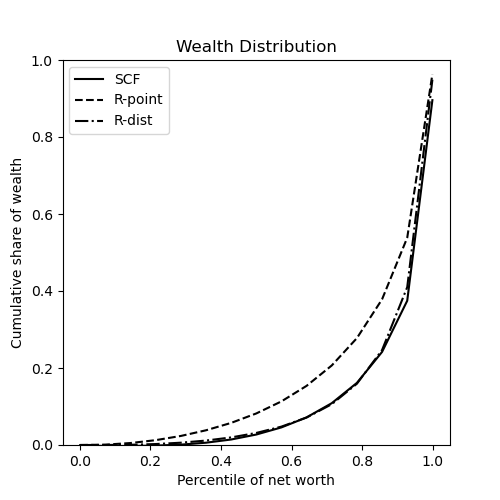
\includegraphics[width=0.7\textwidth]{./Figures/LCUnif.png}
   \caption{Life cycle lorenz curve v.s. data}
    \label{fig:LCUnif}
  \end{figure}\unskip

\onlyinsubfile{% Allows two (optional) supplements to hard-wired \texname.bib bibfile:
% system.bib is a default bibfile that supplies anything missing elsewhere
% Add-Refs.bib is an override bibfile that supplants anything in \texfile.bib or system.bib
\provideboolean{AddRefsExists}
\provideboolean{systemExists}
\provideboolean{BothExist}
\provideboolean{NeitherExists}
\setboolean{BothExist}{true}
\setboolean{NeitherExists}{true}

\IfFileExists{\econtexRoot/Add-Refs.bib}{
  % then
  \typeout{References in Add-Refs.bib will take precedence over those elsewhere}
  \setboolean{AddRefsExists}{true}
  \setboolean{NeitherExists}{false} % Default is true
}{
  % else
  \setboolean{AddRefsExists}{false} % No added refs exist so defaults will be used
  \setboolean{BothExist}{false}     % Default is that Add-Refs and system.bib both exist
}

% Deal with case where system.bib is found by kpsewhich
\IfFileExists{/usr/local/texlive/texmf-local/bibtex/bib/system.bib}{
  % then
  \typeout{References in system.bib will be used for items not found elsewhere}
  \setboolean{systemExists}{true}
  \setboolean{NeitherExists}{false}
}{
  % else
  \typeout{Found no system database file}
  \setboolean{systemExists}{false}
  \setboolean{BothExist}{false}
}

\ifthenelse{\boolean{showPageHead}}{ %then
  \clearpairofpagestyles % No header for references pages
  }{} % No head has been set to clear

\ifthenelse{\boolean{BothExist}}{
  % then use both
  \typeout{bibliography{\econtexRoot/Add-Refs,\econtexRoot/\texname,system}}
  \bibliography{\econtexRoot/Add-Refs,\econtexRoot/\texname,system}
  % else both do not exist
}{ % maybe neither does?
  \ifthenelse{\boolean{NeitherExists}}{
    \typeout{bibliography{\texname}}
    \bibliography{\texname}}{
    % no -- at least one exists
    \ifthenelse{\boolean{AddRefsExists}}{
      \typeout{bibliography{\econtexRoot/Add-Refs,\econtexRoot/\texname}}
      \bibliography{\econtexRoot/Add-Refs,\econtexRoot/\texname}}{
      \typeout{bibliography{\econtexRoot/\texname,system}}
      \bibliography{        \econtexRoot/\texname,system}}
  } % end of picking the one that exists
} % end of testing whether neither exists
}

\ifthenelse{\boolean{Web}}{}{
  \onlyinsubfile{\captionsetup[figure]{list=no}}
  \onlyinsubfile{\captionsetup[table]{list=no}}
}
\end{document}	\endinput

